\documentclass[dvipdfmx,a4j]{jbook}
\usepackage{wrapfig}
\usepackage{tikz}
\usetikzlibrary{shapes,calc,arrows.meta}
\usepackage{amsmath}
\usepackage{amssymb}
\usepackage{fancyvrb}
\usepackage{tabularx}
%\graphicspath{{figs241004/}}
\usepackage{here}
\usepackage{graphicx}
\usepackage{fancyvrb}
\usepackage{multirow}
%\include{mymacros}
\usepackage{subfig}
%\usepackage[framemethod=tikz]{mdframed}
\newcounter{coffee}
\newcounter{bean}
\usepackage{docmute}
\usepackage{url}
\usepackage{makeidx}
\usepackage{here}
\usepackage{array}
\usepackage{tabularx}
\usepackage{mdframed}
\usepackage{longtable}
\newtheorem{Def}{定義}[chapter]
\newtheorem{Thm}{定理}[chapter]
\newtheorem{Prop}{命題}[chapter]
\newtheorem{Lem}{補題}[chapter]
\newtheorem{Exmp}{例}[chapter]
\newtheorem{Alg}{アルゴリズム}[chapter]

\newtheorem*{repeatedtheorem}{定理 \repeatednumber}
\newtheorem*{repeatedlemma}{補題 \repeatednumber}

\renewcommand{\proofname}{証明}

\newenvironment{repThm}[1]
{\def\repeatednumber{\ref{#1}}\begin{repeatedtheorem}}
{\end{repeatedtheorem}}

\newenvironment{repLem}[1]
{\def\repeatednumber{\ref{#1}}\begin{repeatedlemma}}
{\end{repeatedlemma}}

\newcommand{\tuple}[1]{\langle{#1}\rangle}
\newcommand{\Term}[1]{`\mbox{$\mathtt{#1}$}'}
\newcommand{\NTerm}[1]{\tuple{\mbox{$\mathsf{#1}$}}}
\newcommand{\First}[1]{\mathsf{First}_1({#1})}
\newcommand{\Follow}[1]{\mathsf{Follow}_1({#1})}
\newcommand{\greentext}[1]{{\color[rgb]{0,0.5,0}{#1}}}
\newcommand{\bluetext}[1]{{\color{blue}{#1}}}

\newcommand{\eof}{{\tt \#}}
\newcommand{\ttpl}{{\tt +}}
\newcommand{\ttsb}{{\tt -}}
\newcommand{\ttmu}{{\tt *}}
\newcommand{\ttdv}{{\tt /}}
\newcommand{\ttlp}{{\tt (}}
\newcommand{\ttrp}{{\tt )}}
\newcommand{\tteq}{{\tt =}}
\newcommand{\ttlt}{{\tt <}}
\newcommand{\ttcm}{{\tt ,}}

\newcommand{\ttbrkl}{{\tt [}}
\newcommand{\ttbrkr}{{\tt ]}}

\newcommand{\ttif}{{\tt if}}
\newcommand{\ttfi}{{\tt fi}}
\newcommand{\ttthen}{{\tt then}}
\newcommand{\ttelse}{{\tt else}}
\newcommand{\ttwhile}{{\tt while}}
\newcommand{\ttdo}{{\tt do}}
\newcommand{\ttod}{{\tt od}}

\newcommand{\ttassgn}{{\tt :=}}
\newcommand{\ttsc}{{\tt ;}}

\newcommand{\ttand}{{\tt \&\&}}
\newcommand{\ttor}{{\tt ||}}
\newcommand{\ttneg}{{\tt !}}

\newcommand{\tti}{\texttt{i}}
\newcommand{\ttj}{\texttt{j}}
\newcommand{\ttk}{\texttt{k}}
\newcommand{\ttx}{\texttt{x}}
\newcommand{\tty}{\texttt{y}}
\newcommand{\ttz}{\texttt{z}}

\newcommand{\rppush}[1]{\mathsf{push}\ \texttt{#1}}
\newcommand{\rpassign}{{\tt :=}}
\newcommand{\rpframe}[1]{\draw #1 -- ($#1+(0,1)$) #1 -- ($#1+(1.5,0)$) ($#1+(1.5,0)$) -- ($#1+(1.5,1)$);}
\newcommand{\rpframerow}[2]{\draw ($#1}

\newcommand{\newTemp}[1]{{\tt newTemp(}#1\texttt{)}}
\newcommand{\newTempnull}{{\tt newTemp}}
\newcommand{\newLabel}[1]{{\tt newLabel(}#1\texttt{)}}
\newcommand{\newLabelnull}{{\tt newLabel}}
\newcommand{\generatefo}[4]{{\tt generate(}{#1},=,{#2},{#3},{#4}\texttt{)}}
\newcommand{\generateth}[3]{{\tt generate(}{#1},=,{#2},{#3}\texttt{)}}
\newcommand{\generatetw}[2]{{\tt generate(}{#1},=,{#2}\texttt{)}}
\newcommand{\generateon}[1]{{\tt generate(}{#1}\texttt{)}}
\newcommand{\generateCTL}[3]{{\tt generate(}{#1}.{#2},{#3}\texttt{)}}
\newcommand{\generate}[1]{{\tt generate(}{#1}{\tt )}}
\newcommand{\generatenull}{{\tt generate}}
\newcommand{\generateassgin}[2]{{\tt generate}(`{#1}{\tt =}{#2}')}
\newcommand{\generateif}[2]{{\tt generate}(`{\tt if}\ {#1}\ {\tt goto}\ {#2}')}
\newcommand{\generateifnot}[2]{{\tt generate}(`{\tt if\_not}\ {#1}\ {\tt goto}\ {#2}')}
\newcommand{\generatelabel}[1]{{\tt generate(`label\ }{#1}')}
\newcommand{\generategoto}[1]{{\tt generate(`goto\ }{#1}')}

\newcolumntype{b}{X}
\newcolumntype{s}{>{\hsize=.5\hsize}X}

\newcolumntype{Y}{>{\centering\arraybackslash}X}
\newcommand{\inst}[1]{\begin{tabularx}{.3\textwidth}{|Y|Y|Y|Y|}\hline\texttt{#1}& $b$ & $i$ &$a$\\\hline\end{tabularx}}
\newcommand{\ignored}[1]{\par #1は無視される。}

\newcommand{\bnfnts}[1]{\langle\mathrm{#1}\rangle}
\newcommand{\bnfts}[1]{\texttt{'#1'}}
\newcommand{\bnfarr}{\texttt{::=}}

\newcommand{\domv}[1]{\mathsf{dom}({#1})}
\newcommand{\idomv}[1]{\mathsf{idom}({#1})}
\newcommand{\domgg}{\underline{\gg}}
\newcommand{\domll}{\underline{\ll}}

\newcommand{\loadinst}[2]{\texttt{Load}\>{$#1$}\>{$#2$}}
\newcommand{\oprinst}[3]{\texttt{#1}\>{#2}\>{#3}}

\setcounter{chapter}{6}
% \setcounter{page}{63}
% \newcounter{coffee}
% \newcounter{bean}
%\graphicspath{{figs241108/}}
\begin{document}
\chapter{コード最適化}

本章では，中間コードのレベルで意味を保ちながらより高速なコードに変換する手法について述べる．
ソースコードから構文的に生成された中間コードは不要な繰り返しや変数間のコピーが多く生成されるため，
制御フローとデータフローを中間コードを解析して同じ効果をもつより効率的なコードに変換する．この
過程を{\bf コード最適化(code optimization)}と呼ぶ．
さらに，最近のコンパイラで用いられている　{\bf 静的単一代入形式(static single assignment, SSA)}を用いた
最適化手法を紹介する．SSAの特徴は，その名前の通り，変数に対する代入を一度に制限して上書きしない．SSAでは，変数がより多く必要になる一方，変数の名前によってデータフローが構文として表現されるため，コンパイラの最適化の際に必要なフロー解析が容易になる．

\section{基本ブロックとフローグラフ}

3番地コードレベルの抽象度を持つ言語の命令の系列に対して，以下の条件を満たす系列を{\bf 基本ブロック}という．

実行制御がその系列の先頭から最後まで，条件付きジャンプおよび無条件ジャンプは最後の場所でのみ出現し，他の命令からのジャンプ先は必ず系列の先頭しかない．

\begin{figure}[H]
    \centering
    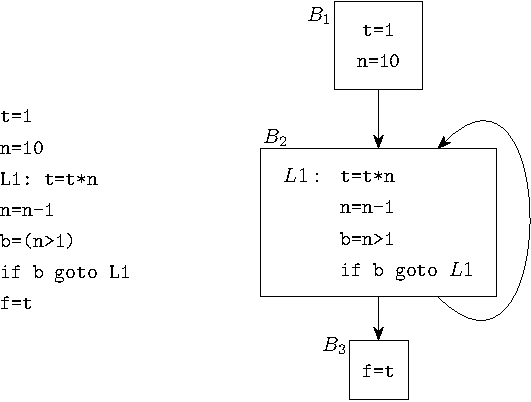
\includegraphics{figures/threeAddressCode-CFG-crop.pdf}
    \caption{3番地コードとそのCFG}\label{flg:flowgraph}
\end{figure}

基本ブロックでは，すべての命令の前提としてそれより前にある命令が必ず実行されている．
３番地コードから構成される基本ブロック内では，参照される変数について，それより前の
ブロック内で定義されていれば，最後に定義されたところの値を持つことがわかる．そうでなければ，
先頭にジャンプしているブロック内の値が引き継がれる．

基本ブロックを頂点として，制御のフローを有向グラフで表した構造を{\bf フローグラフ（あるいは，
    コントロールフローグラフ，CFG）}と呼び．$(V,E,v_{init})$で表す．ここで，$V$は頂点の集合で，
各頂点$v$には基本ブロック$B(v)$が割り当てられている．
$(v_1,v_2)\in E$であるとき，$B(v_1)$の実行後，直ちに$B(v_2)$が実行されることが可能である
ことを表し，$v_1\rightarrow v_2$と書くことにする．$v_{init}\in V$は，フローグラフの実行が
$B(v_{init})$から開始されることを表す．

基本ブロック中では，制御の合流や分岐が存在しないので，
CFGはプログラムの振舞いを抽象的に表現していることになる．

\section{局所最適化}

局所最適化は，3番地コードの系列で構成される基本ブロックに対して同じ意味を持つ
より短くて変数の少ない系列を求める．

\subsection{局所最適化の例}

\subsubsection{定数伝播(constant propagation)}
定数畳み込み(constant folding)とも言う．実行によって値が変わらない変数は，
プログラムとして値を埋め込んでメモリ上の値の参照を減らす．

\begin{center}
    \begin{tabular}{lclp{6cm}}
        $\texttt{a=2*3.14}$ & $\rightarrow$ & $\texttt{a=6.28}$   & 定数計算をコンパイル時に行う．              \\
        $\texttt{b=a/100}$  & $\rightarrow$ & $\texttt{b=0.0628}$ & $\texttt{b}$はコンパイル時に値が決定できる．
    \end{tabular}
\end{center}

変数の値を参照する場合には，メモリから値を読み出す必要があるが，定数にすると値自体を
コードとして生成できるので，高速になる．

\subsubsection{共通部分式削除}

同じ部分式で同じ計算の繰り返しをまとめて，計算の繰り返しを防ぐ．

\begin{center}
    \begin{tabular}{lcl}
        $\texttt{x=a*b}$ &               & $\texttt{x=a*b}$ \\
        $\texttt{y=x+c}$ &               & $\texttt{y=x+c}$ \\
        $\texttt{d=a*b}$ & $\Rightarrow$ & $\texttt{d=x}$   \\
        $\texttt{e=d-c}$ &               & $\texttt{e=d-c}$
    \end{tabular}
\end{center}

以下の系列では，同じ形の部分式$\texttt{b+c}$があるが，$\texttt{a}$
と$\texttt{e}$に対する代入で値が更新されているので，$\texttt{e=a}$の
ような消去はできない．

\begin{center}
    \begin{tabular}{lcl}
        $\texttt{a=b+c}$ &                   & $\texttt{a=b+c}$ \\
        $\texttt{b=b-d}$ &                   & $\texttt{b=b-c}$ \\
        $\texttt{c=c+d}$ &                   & $\texttt{c=c+d}$ \\
        $\texttt{e=b+c}$ & $\not\Rightarrow$ & $\texttt{e=a}$
    \end{tabular}
\end{center}

\subsubsection{コピー伝播}

$\texttt{a=b}$のような変数のコピーがある場合，$a$と$b$は同じ値を保持しているので，$a$を代入する必要はない．

\begin{center}
    \begin{tabular}{lcl}
        $\texttt{a=b}$   &               & $\texttt{a=b}$   \\
        $\texttt{c=a+d}$ & $\Rightarrow$ & $\texttt{c=b+d}$ \\
        $\texttt{e=e-a}$ &               & $\texttt{e=e-b}$
    \end{tabular}
\end{center}

このブロックの後で，$\texttt{a}$が使われることがなければ，$\texttt{a=b}$は
消去しても構わない．基本ブロックで用いられる変数については，データフロー解析など
の手法を用いて求めることができる場合がある．不要コードの消去(Dead-code elimination)
によってより高速にすることができる．

\subsubsection{代数的性質の利用}

\begin{center}
    \begin{tabular}{lcl}
        $\texttt{a+0}$       & $\Rightarrow$ & $\texttt{0}$     \\
        $\texttt{b*1}$       & $\Rightarrow$ & $\texttt{b}$     \\
        $\texttt{1+(c+2)}$   & $\Rightarrow$ & $\texttt{3+c}$   \\
        $\texttt{d*(1+e/d)}$ & $\Rightarrow$ & $\texttt{d+e}$   \\
        $\texttt{x*2}$       & $\Rightarrow$ & $\texttt{x+x}$   \\
        $\texttt{x/5}$       & $\Rightarrow$ & $\texttt{x*0.2}$ \\
    \end{tabular}
\end{center}

演算の単位元などによる簡単化，分配則による簡単化などによって式を短縮化する．
さらに命令を低レベルのマシン語に変換するときに，除算よりも積算，積算よりも和算
の方がサイクルが少ないので，より軽い命令に変更することで高速化が期待できる．

局所最適化については，個々の最適化について大きな効果は期待できない．
しかし，基本ブロックがループによって繰り返し実行されるとプログラム全体では
大きな効果が期待できる．

\subsection{基本ブロックのDAG表現}

基本ブロックを有向非巡回グラフ(Directed Acyclic Graph, DAG)を用いて
表すことによって，各３番地コードにおける参照関係を表現できる．参照関係を
壊さない等価なグラフの変形によって最適化を行う．基本ブロックに対して，
以下のアルゴリズムによってDAGを生成する．

\begin{Alg}
    DAGの頂点が始点となる辺を持たない頂点を葉頂点と呼ぶ．葉頂点には，変数
    または定数のラベルをつける．葉以外の頂点には，演算$\theta$と，演算の
    結果が収納される変数のラベルのリストをつける．
    \begin{enumerate}
        \item 基本ブロックに入る前に定義された値を参照する変数名と定数値に対して，
              葉頂点を生成し，変数$x$に対して，$x_0$を頂点にラベルづけし，$[x]$を変数
              リストとする．定数$c$に対しては，$c$を頂点にラベル付けする．
        \item 基本ブロック内のすべての代入文について上から順に以下の操作を適用する．
              \begin{list}{}{}
                  \item [(a)]
                        代入文$X=A\theta B$に対して，$A$,$B$が変数であるときは変数ラベルに持つ
                        頂点を$v_A$, $v_B$とする．定数の場合は定数をラベルにもつ
                        $v_A$, $v_B$を選ぶ．
                  \item [(b)] $X$を変数リストに含む頂点があれば，その変数リストから$X$を削除する．
                  \item [(c)] $v_A$, $v_B$を子に持ち，$\theta$を演算ラベルとする
                        ノード$v_\theta$がすでに存在するならば，$v_\theta$の変数リストに$X$を追加する．
                        $v_\theta$が存在しないならば，$v_\theta$を新たに生成して，$v_A$, $v_B$を子ノードとする辺を追加し，$\theta$を$v_\theta$の演算ラベルとし，$[X]$を変数リストとする．
                  \item [(d)] $X=A$の場合は，すでに存在する頂点の変数リストに$X$が含まれれば，消去した上で，$v_A$の変数リストに$X$を追加する．
              \end{list}
    \end{enumerate}
\end{Alg}

\begin{Exmp}\label{example:DAG}
    以下にアルゴリズムで生成されるDAGを示す．５行の基本ブロックにおいて，
    最初の３行までで，まず(a)に示すDAGが生成される．
    \begin{center}
        \begin{tabular}{ccc}
            \begin{tikzpicture}
                \node[draw,circle,label={180:$[\texttt{a}]$}] (A0) at (0,0) {$a_0$};
                \node[draw,circle,label={0:$[\texttt{b}]$}] (B0) at (1,0) {$b_0$};
                \node[draw,circle,label={0:$[\texttt{c}]$}] (C0) at (2,1) {$c_0$};
                \node[draw,circle,label={180:$[\texttt{x},\texttt{d}]$}] (X1) at (0.5,1) {$\texttt{*}$};
                \node[draw,circle,label={180:$[\texttt{y}]$}] (Y1) at (1.25,2) {$\texttt{+}$};
                \path[->] (X1) edge (A0) (X1) edge (B0);
                \path[->] (Y1) edge (X1) (Y1) edge (C0);
            \end{tikzpicture}
             &  &
            \begin{minipage}{.2\linewidth}
                \vspace*{-2cm}
                \begin{Verbatim}
                    x=a*b
                    y=x+c
                    d=a*b
                \end{Verbatim}
            \end{minipage}          \\
            \multicolumn{3}{c}{(a) ３行目までで生成されるDAG} \\[5mm]
            \begin{tikzpicture}
                \node[draw,circle,label={180:$[\texttt{a}]$}] (A0) at (0,0) {$a_0$};
                \node[draw,circle,label={0:$[\texttt{b}]$}] (B0) at (1,0) {$b_0$};
                \node[draw,circle,label={0:$[\texttt{c}]$}] (C0) at (2,1) {$c_0$};
                \node[draw,circle,label={180:$[\texttt{d}]$}] (X1) at (0.5,1) {$\texttt{*}$};
                \node[draw,circle,label={180:$[\texttt{y}]$}] (Y1) at (1.25,2) {$\texttt{+}$};
                \node[draw,circle,label={180:$[\texttt{e}]$}] (E1) at (1.25,3) {$\texttt{-}$};
                \node[draw,circle,label={180:$[\texttt{x}]$}] (X2) at (0.35,4) {$\texttt{+}$};
                \path[->] (X1) edge (A0) (X1) edge (B0);
                \path[->] (Y1) edge (X1) (Y1) edge (C0);
                \path[->] (E1) edge (X1) (E1) edge (C0);
                \path[->] (X2) edge (X1) (X2) edge (E1);
            \end{tikzpicture}
             &  &
            \begin{minipage}{.2\linewidth}
                \vspace*{-3cm}
                \begin{Verbatim}
                    x=a*b
                    y=x+c
                    d=a*b
                    e=d-c
                    x=d+e
                \end{Verbatim}
            \end{minipage}          \\
            \multicolumn{3}{c}{(b) 5行目までで生成されるDAG}
        \end{tabular}
    \end{center}
    ４行目の命令でさらに$\texttt{e}$に対するノードが新たに生成され，
    ５行目では$\texttt{x}$が更新されるため，既存の変数リストから
    $\texttt{x}$を消去して新しく一番上のノードに$\texttt{x}$を変数
    リストに追加している．

    例\ref{example:DAG}の(a)において，$[\texttt{x},\texttt{d}]$のように
    複数の変数が一つのノードにつけられる場合は，共通部分式が存在するということであるので
    共有部分式の消去が適用できる．さらに，コピー伝播を適用すると(c)のようになる．

    \begin{center}
        \begin{tabular}{ccc}
            \begin{tikzpicture}
                \node[draw,circle,label={180:$[\texttt{a}]$}] (A0) at (0,0) {$a_0$};
                \node[draw,circle,label={0:$[\texttt{b}]$}] (B0) at (1,0) {$b_0$};
                \node[draw,circle,label={0:$[\texttt{c}]$}] (C0) at (2,1) {$c_0$};
                \node[draw,circle,label={180:$[\texttt{d}]$}] (X1) at (0.5,1) {$\texttt{*}$};
                \node[draw,circle,label={180:$[\texttt{y}]$}] (Y1) at (1.25,2) {$\texttt{+}$};
                \node[draw,circle,label={180:$[\texttt{e}]$}] (E1) at (1.25,3) {$\texttt{-}$};
                \node[draw,circle,label={180:$[\texttt{x}]$}] (X2) at (0.35,4) {$\texttt{+}$};
                \path[->] (X1) edge (A0) (X1) edge (B0);
                \path[->] (Y1) edge (X1) (Y1) edge (C0);
                \path[->] (E1) edge (X1) (E1) edge (C0);
                \path[->] (X2) edge (X1) (X2) edge (E1);
            \end{tikzpicture}
             &  &
            \begin{minipage}{.2\linewidth}
                \vspace*{-3cm}
                \begin{Verbatim}
                    x=a*b
                    y=x+c
                    d=x
                    e=x-c
                    x=x+e
                \end{Verbatim}
            \end{minipage} \\
            \multicolumn{3}{c}{(c) 共有部分式とコピー伝播の適用}
        \end{tabular}
    \end{center}

    この基本ブロックの後で$\texttt{y}$が使われない場合は，$[\texttt{y}]$を
    変数リストにもつ頂点とその辺を消去しても意味は変わらない．これに対して，
    $\texttt{d}$が使われない場合は，$[\texttt{d}]$の頂点を消すことはできない．
    これは，$\texttt{x}$が$\texttt{d}$の頂点に依存しているためである．

    \begin{center}
        \begin{tabular}{ccc}
            \begin{tikzpicture}
                \node[draw,circle,label={180:$[\texttt{a}]$}] (A0) at (0,0) {$a_0$};
                \node[draw,circle,label={0:$[\texttt{b}]$}] (B0) at (1,0) {$b_0$};
                \node[draw,circle,label={0:$[\texttt{c}]$}] (C0) at (2,1) {$c_0$};
                \node[draw,circle,label={180:$[\texttt{d}]$}] (X1) at (0.5,1) {$\texttt{*}$};
                \node[draw,circle,label={180:$[\texttt{e}]$}] (E1) at (1.25,3) {$\texttt{-}$};
                \node[draw,circle,label={180:$[\texttt{x}]$}] (X2) at (0.35,4) {$\texttt{+}$};
                \path[->] (X1) edge (A0) (X1) edge (B0);
                \path[->] (E1) edge (X1) (E1) edge (C0);
                \path[->] (X2) edge (X1) (X2) edge (E1);
            \end{tikzpicture}
             &  &
            \begin{minipage}{.2\linewidth}
                \vspace*{-3cm}
                \begin{Verbatim}
                    x=a*b
                    d=x
                    e=x-c
                    x=x+e
                \end{Verbatim}
            \end{minipage} \\
            \multicolumn{3}{c}{(d) 不要コード消去の適用}
        \end{tabular}
    \end{center}
\end{Exmp}

\section{大域最適化}

複数の基本ブロックにわたる最適化を大域的最適化とよぶ．この最適化を行うために，
フローグラフの構造にマッチする構造を見つける方法について示す．

\subsection{意味等価な変換}

プログラムにおいて，全体の１，２割の部分が，実際の実行の８，９割の時間を占める．これは，
プログラムの一部がループ構造になって繰り返し実行されることによる．繰り返しに含まれる
基本ブロックを局所最適化によって最適化することによって大きな効果が期待できることは
述べた．これに加えて，ループ構造として最適化する手法について示す．

ループ構造の最適化は，制御フローグラフに依存するため，ソースコードでも３番地コードでも
ほぼ変わらない．以下では，C言語プログラムの一部で最適化の手法について示す．


\subsubsection{ループ最適化}

\paragraph{ループ不変コードの移動}

ループ内で値が変化しない変数をループの外に移動し，計算に影響しない命令が何度も実行されずに
同じ意味を表現するようにする．

\begin{center}
    \begin{tabular}{ccc}
        \begin{minipage}{.3\linewidth}
            \begin{Verbatim}
                i=1;
                do {
                        c=a/b;x=i*c; .... i++;
                    } while(i<n);
            \end{Verbatim}
        \end{minipage}
         & $\Rightarrow$ &
        \begin{minipage}{.3\linewidth}
            \begin{Verbatim}
                i=1;t=a/b;
                do {
                        c=t;x=i*c;...i++;
                    } while(i<n);
            \end{Verbatim}
        \end{minipage}
    \end{tabular}
\end{center}

$\texttt{do}$ ... $\texttt{while}$で，$\texttt{a}$, $\texttt{b}$のいずれも
更新されないとき，$\texttt{c}$はループ実行で変化しないため，ループ外で値を一度代入する
同じ計算となる．

\begin{center}
    \begin{tabular}{ccc}
        \begin{minipage}{.3\linewidth}
            \begin{Verbatim}
                for(i=1;i<n;i++) {
                        c=a/b;x=i*c;...
                    }
            \end{Verbatim}
        \end{minipage}
         & $\Rightarrow$ &
        \begin{minipage}{.3\linewidth}
            \begin{Verbatim}
                if(n>1) {
                        t=a/b;
                        for(i=1;i<n;i++) {
                                c=t;x=i*c;...
                            }
                    }
            \end{Verbatim}
        \end{minipage}
    \end{tabular}
\end{center}
一般的な{\tt for}ループでは，条件によってループの内容が実行されないこともあるため，
不変コードはループが実行された場合だけ，実行されるように変換する必要がある．

\paragraph{ループ内演算の強さ軽減}

\begin{center}
    \begin{tabular}{ccc}
        \begin{minipage}{.3\linewidth}
            \begin{Verbatim}
                for(i=1;i<n;i++)
                a=a+b*i;
            \end{Verbatim}
        \end{minipage}
         & $\Rightarrow$ &
        \begin{minipage}{.3\linewidth}
            \begin{Verbatim}
                t=0;
                for(i=1;i<n;i++) {
                        t=t+b;a=a+t;
                    }
            \end{Verbatim}
        \end{minipage}
    \end{tabular}
\end{center}

\paragraph{帰納変数の消去}

\begin{center}
    \begin{tabular}{ccc}
        \begin{minipage}{.3\linewidth}
            \begin{Verbatim}
                t=b;
                for(i=1;i<n;i++) {
                        a=a+t;t=t+b;
                    }
            \end{Verbatim}
        \end{minipage}
         & $\Rightarrow$ &
        \begin{minipage}{.3\linewidth}
            \begin{Verbatim}
                m=n*b;
                for(t=b;t<m;t=t+b)
                a=a+t;
            \end{Verbatim}
        \end{minipage}
    \end{tabular}
\end{center}

\paragraph{ループ融合}

\begin{center}
    \begin{tabular}{ccc}
        \begin{minipage}{.3\linewidth}
            \begin{Verbatim}
                for(i=1;i<n;i++)
                a[i+1]=a[i]+i;
                for(i=1;i<n;i++)
                b[i]=a[i]+i;
            \end{Verbatim}
        \end{minipage}
         & $\Rightarrow$ &
        \begin{minipage}{.3\linewidth}
            \begin{Verbatim}
                for(i=1;i<n;i++) {
                        a[i+1]=a[i]+i;
                        b[i]=a[i]+i;
                    }
            \end{Verbatim}
        \end{minipage}
    \end{tabular}
\end{center}

\paragraph{ループ分解}

\begin{center}
    \begin{tabular}{ccc}
        \begin{minipage}{.3\linewidth}
            \begin{Verbatim}
                for(i=1;i<n;i++) {
                        a[i+1]=a[i]+i;
                        b[i]=a[i]+i;
                    }
            \end{Verbatim}
        \end{minipage}
         & $\Rightarrow$ &
        \begin{minipage}{.3\linewidth}
            \begin{Verbatim}
                for(i=1;i<n;i++)
                a[i+1]=a[i]+i;
                for(i=1;i<n;i++)
                b[i]=a[i]+i;
            \end{Verbatim}
        \end{minipage}
    \end{tabular}
\end{center}

\paragraph{ループ展開}

\begin{center}
    \begin{tabular}{ccc}
        \begin{minipage}{.3\linewidth}
            \begin{Verbatim}
                for(i=1;i<n;i++) {
                        a[i+1]=a[i]+i;
                        b[i]=a[i]+b[i-1];
                    }
            \end{Verbatim}
        \end{minipage}
         & $\Rightarrow$ &
        \begin{minipage}{.3\linewidth}
            \begin{Verbatim}
                for(i=1;i<n;i++) {
                        a[i]=a[i-1]+i;
                        b[i]=a[i]+b[i-1];a[i+1]=a[i]+1;
                        b[i+1]=a[i+1]+b[i];
                    }
            \end{Verbatim}
        \end{minipage}
    \end{tabular}
\end{center}

\paragraph{ソフトウェアパイプライン}

\begin{center}
    \begin{tabular}{ccc}
        \begin{minipage}{.3\linewidth}
            \begin{Verbatim}
                for(i=1;i<1000;i++) {
                        a[i]=a[i-1]+1; // Ai
                        b[i]=a[i]+b[i-1]; // Bi
                        c[i]=b[i]+2; // Ci
                    }
            \end{Verbatim}
        \end{minipage}
         & $\Rightarrow$ &
        \begin{minipage}{.3\linewidth}
            \begin{Verbatim}
                A1;
                B1; A2;
                for(i=3;i<1000;i++) {
                        Ci-2;Bi-1;Ai;
                    }
                C998;B999;
                C999;
            \end{Verbatim}
        \end{minipage}
    \end{tabular}
\end{center}

\subsubsection{手続き呼び出し最適化}

\paragraph{インライン展開}

手続き呼び出しは，スタック上に局所環境を作成し，リターンの際にもスタック上の局所環境をクリアする
必要がある．局所環境を作成するほどでもない単純な手続き呼び出しでは，スタック操作を行わなくても
よい場合もあり，ループ構造内では大きな高速化の効果が期待できる．

\begin{center}
    \begin{tabular}{ccc}
        \begin{minipage}{.3\linewidth}
            \begin{Verbatim}
                int square(int x) {
                        return x*x;
                    }
                y = square(a);
            \end{Verbatim}
        \end{minipage}
         & $\Rightarrow$ &
        \begin{minipage}{.3\linewidth}
            \begin{Verbatim}
                y = a * a;
            \end{Verbatim}
        \end{minipage}
    \end{tabular}
\end{center}

c言語では，関数の前に{\tt inline}を付加することでスタックを用いずに呼び出しを
行う．ただし，{\tt inline}をつけた場合は，実際にインライン展開するかどうかは
コンパイラで判断する．必ず展開する場合は，{\verb|#define|}でマクロ定義すれば
呼び出しと同様の形式でプログラムを記述できる．

\paragraph{末尾再帰}

再帰呼び出しは，呼び出し定義の中で自分を呼び出すことである．
定義の中の呼び出しが定義の最後の命令であるとき，関数からリターンしたあと
もとの環境の変数は参照されないので，環境を復元する必要がない．従って，
インラインでない関数呼び出しを行う場合であっても，毎回，局所環境を作成する
必要がなく，最初の１回目の呼び出しで作成した領域を上書きすればよい．
変換としては，再帰呼び出しをgotoに置き換えることで高速化が可能である．

\begin{center}
    \begin{tabular}{ccc}
        \begin{minipage}{.4\linewidth}
            \begin{Verbatim}
                int sum_tail(int n, int acc) {
                        if (n == 0) {
                                return acc;
                            }
                        return sum_tail(n-1,acc+n);
                    }
            \end{Verbatim}
        \end{minipage}
         & $\Rightarrow$ &
        \begin{minipage}{.4\linewidth}
            \begin{Verbatim}
                int sum_tail(int n, int acc) {
                        L:  if (n == 0) {
                                return acc;
                            }
                        acc+=n; n--;
                        goto L;
                    }
            \end{Verbatim}
        \end{minipage}
    \end{tabular}
\end{center}
gotoによるループ構造をgotoなしで記述すると以下のプログラムと等価である．

\begin{center}
    \begin{minipage}{.3\linewidth}
        \begin{Verbatim}
            int sum(int n,int acc) {
                    while(n!=0) {
                            acc+=n; n--;
                        }
                    return acc;
                }
        \end{Verbatim}
    \end{minipage}
\end{center}

\subsection{データフロー解析}

プログラムの実行意味が状態遷移に基づいて決まるとすると，プログラムの状態を決定する
変数の実行に従った更新（{\bf データフロー}）を解析することでプログラムの
実行意味を
捉えることが可能になる．基本ブロックを越えて最適化を行うためには，フローグラフ上で
各基本ブロックにどの変数が入力されてどの変数を出力するか，ということを解析して，
代入された値がどこまで参照として有効か（定義到達解析），以降の実行でどこまでその
変数が用いられるか（生存解析），同じ値を計算する式の検出（利用可能式解析）などの
解析手法が用いられる．このような解析はプログラムを実行することなく行われるため，
{\bf 静的解析}という．この解析において，一般にプログラムの成魚がループを
持つことから変数の更新は自身の更新に依存するため，この解析においては
データフロー方程式を解く必要が生じる．

\subsubsection{定義到達解析}

定義到達解析は，$v\texttt{=}E$という形の３番地コードは$v$を定義しているとし，
ここで定義された$v$の値がどこまで変更されずに到達するか，ということを
解析する．$v$が別の命令で上書きされるとき，先の定義はkillされる．
各定義の３番地命令にラベル$d_i$をつけ，基本ブロック$B$ごとに
以下の定義ラベルの集合を定める．
\begin{list}{$\cdot$}{}
    \item $Gen[B]$: $B$のなかで定義され，上書きされない定義の集合
    \item $Kill[B]$ $B$のなかで上書きされる定義の集合
    \item $In[B]$ $B$が実行される際に参照する変数に対する定義の集合
    \item $Out[B]$ $B$が実行された後に有効な定義の集合
\end{list}
ここで$Gen$, $Kill$は定義の実行順は関係なく，定義集合全体に
対して定める．

基本ブロックから構成されるフローグラフが与えられたとき，以下の関係がある．
\begin{eqnarray}
    In[B] & = & \cup_{P\in\mathsf{Pred}(B)}Out[P]\\
    Out[B] & = & Gen[B]\cup (In[B]\backslash Kill[B])
\end{eqnarray}
ここで，$\mathsf{Pred}(B)$は，フローグラフにおいて，$B$の先行頂点
(predecessor)の集合を表す．基本ブロック内では，制御の分岐はない．
基本ブロックには，その直是のブロックから出力されるフローが入力され，
ブロックからの出力フローは，ブロック内で新たに発生した定義と，入力定義
のうちkillされなかった定義となる．

図\ref{fig:flowgraph}のコードにおいて以下のように定義のラベル付けをする．
\[
    \begin{array}{rrl}
        d_1: &     & \texttt{t=1}          \\
        d_2: &     & \texttt{n=10}         \\
        d_3: & L1: & \texttt{t=t*n}        \\
        d_4: &     & \texttt{n=n-1}        \\
        d_5: &     & \texttt{b=(n>1)}      \\
             &     & \texttt{if b goto }L1 \\
        d_6: &     & \texttt{f=t}          \\
    \end{array}
\]
$B_i$に対する$Gen$, $Kill$は以下のようになる．
\begin{trivlist}
    \item $Gen[B_1]=\{d_1,d_2\}$, $Kill[B_1]=\{d_3,d_4\}$
    \item $Gen[B_2]=\{d_3,d_4,d_5\}$, $Kill[B_2]=\{d_1,d_2\}$
    \item $Gen[B_3]=\{d_6\}$, $Kill[B_3]=\varnothing$
\end{trivlist}
$In$, $Out$については以下の関係がなりたつ．
\begin{trivlist}
    \item $In[B_1]=\varnothing$, $Out[B_1]=Gen[B_1]=\{d_1,d_2\}$
    \item $In[B_2]=Out[B_1]\cup Out[B_2]$, $Out[B_2]=\{d_3,d_4,d_5\}\cup(In[B_2]\backslash\{d_1,d_2\})$
    \item $In[B_3]=Out[B_2]$, $Out[B_3]=\{d_6\}\cup(In[B_2]\backslash\{d_6\})$
\end{trivlist}
$In[B_2]$についての式を代入すると，
\[In[B_2]=\{d_1,d_2\}\cup(\{d_3,d_4,d_5\}\cup(In[B_2]\backslash\{d_1,d_2\}))\]となる．$In[B_2]=X$とおくと，
$X=\{d_1,d_2,d_3,d_4,d_5\}\cup (X\backslash\{d_1,d_2\})$を満たす$X$を
求める必要がある．これを解くには，$X_0=\varnothing$として，
$X_{i+1}=\{d_1,d_2,d_3,d_4,d_5\}\cup (X_i\backslash\{d_1,d_2\})$
で，$X_{i+1}=x_i$となるまで繰り返す．

$X_1=\{d_1,d_2,d_3,d_4,d_5\}$, $X_2=\{d_1,d_2,d_3,d_4,d_5\}$となるので
$X=\{d_1,d_2,d_3,d_4,d_5\}$が条件を満たす．したがって，$Out[B_2]=\{d_3,d_4,d_5\}$，$out[B_3]=\{d_3,d_4,d_5,d_6\}$である．

この解析によってこのプログラムが終了した時点での，$\texttt{t},\texttt{n}$の
有効な定義は，$d_3$および$d_4$であり，$d_1$, $d_2$の定義は伝播しないという
ことがわかる．また，$In[B_2]$において，$\texttt{t}$, $\texttt{n}$に
対する定義は一意的に定まらないので，$B_2$中でそれらの変数を定数に置き換えることは
できないこともわかる．

\subsubsection{生存変数解析}

基本ブロック$B$において，$In[B]$に含まれる定義の変数がKillされる前に
参照されるとき，その定義は$B$で実際に使用される．この変数の集合を$Use[B]$
とする．$B$の中で定義される変数の集合を$Def[B]$とすると，以下の関係が
成り立つ．
\begin{eqnarray}
    In[B] & = & Use[B]\cup(Out[B]\backslash Def[B])\label{eqn:lvin}\\
    Out[B] & = & \cup_{S\in\mathsf{Succ}(B)}In[S]\label{eqn:lvout}
\end{eqnarray}
ここで，$\mathsf{Succ}(B)$はフローグラフでの$B$の後続頂点集合である．

図\ref{flg:flowgraph}について，生存変数解析は以下のようになる．
\begin{trivlist}
    \item $Use[B_1]=\varnothing$, $Def[B_1]=\{t,n\}$
    \item $Use[B_2]=\{t,n\}$, $Def=\{t,n,b\}$
    \item $Use[B_3]=\{t\}$, $Def[B_3]=\{f\}$
\end{trivlist}
(\ref{eqn:lvin})(\ref{eqn:lvout})を適用する．

\begin{trivlist}
    \item $In[B_1]=Out[B_1]\backslash\{t,n\}$, $Out[B_1]=In[B_2]$
    \item $In[B_2]=\{t,n\}\cup(Out[B_2]\backslash\{t,n,b\})$, $Out[B_2]=In[B_2]\cup In[B_3]$
    \item $In[B_3]=\{t\}\cup(Out[B_3]\backslash\{f\})$,$Out[B_3]=\varnothing$
\end{trivlist}

$In$, $Out$は出口から計算できる．$In[B_3]=\{t\}$
$Out[B_2]=In[B_2]\cup\{t\}$,
$In[B_2]=\{t,n\}\cup((In[B_2]\cup\{t\})\backslash\{t,n,b\})$
$In[B_2]=X$とすると，$X=\{t,n\}\cup(X\backslash\{n,b\})$となる．
$X_0=\varnothing$として$X_{i+1}=\{t,n\}\cup(X_i\backslash\{n,b\})$
に代入すると$X_1=\{t,n\}$, $X_2=\{t,n\}$となる．
よって，$Out[B_2]=\{t,n\}$, $Out[B_1]=\{t,n\}$, $In[B_1]=\varnothing$
と決定できる．

生存変数解析によって，基本ブロックの実行の後で使用されない変数を特定できる．
この解析に基づいて使われない変数の計算を基本ブロックから消去することができる．

図\ref{flg:flowgraph}に対する利用可能式解析は以下のようになる．
\begin{trivlist}
    \item $Gen[B_1]=\varnothing$, $Kill[B_1]=\{\texttt{t*n},\texttt{n-1},\texttt{n>1}\}$
    \item $Gen[B_2]=\{\texttt{n>1}\}$, $Kill[B_2]=\{\texttt{t*n},\texttt{n-1},\texttt{n>1}\}$
    \item $Gen[B_3]=\varnothing$, $Kill[B_3]=\varnothing$
\end{trivlist}

IN,OUTは以下のようになる．
\begin{trivlist}
    \item $IN[B_1]=\varnothing$, $OUT[B_1]=\varnothing$
    \item $IN[B_2]=OUT[B_1]\cap OUT[B_2]=\varnothing$
    $OUT[B_2]=\{\texttt{n>1}\}$
    \item $IN[B_3]=OUT[B_2]=\{\texttt{n>1}\}$, $OUT[B_3]=\{\texttt{n>1}\}$
\end{trivlist}

実際に利用可能解析は，配列のアドレス計算において\texttt{a[i]}のデータにアクセスするのに$\texttt{a}$のアドレス計算に$\texttt{i*4}$を計算する場合などに有効である．

\subsubsection{利用可能式解析}

$v\;=\;a\;\texttt{+}\;b$という代入コードがある場合，この基本ブロックの後で
$a\;\texttt{+}\;b$という式が出現しているとき$a$, $b$の値が更新されて
いなければ，計算の重複を避けることが可能になる．変数や定義の代わりに評価式を
蓄積する．式はその要素が一つでも更新されるとkillされる．各基本ブロック$B$
について，$B$の中において計算された後$B$を抜けるまでにkillされることのない
式の集合を$Gen[B]$，$B$の中でkillされる式の集合を$Kill[B]$とする．
ここでは，以下の関係が成り立つ．
\begin{eqnarray}
    IN[B] & = & \cap_{\mathsf{Pred}[B]}Out[P]\\
    OUT[B] & = & Gen[B]\cup(In[B]\backslash Kill[B])
\end{eqnarray}



% \begin{trivlist}
% \item 
% \end{trivlist}

\section{静的単一代入形式と最適化}

最近のコンパイラにおける最適化では，静的単一代入形式(Static single assignment, SSA)を用いる
事が多い．SSA形式では中間コード列の中に各変数の定義（３番地コードの場合は代入の左辺）が一箇所しか
現れないという制約を持つ．定義が１つしかないため，どこで定義された変数がどこで参照されるかが，
プログラムとして明示される．プログラムを解析すれば，プログラムの構文情報からデータフローを
解析することができる．

\subsection{例}

C言語をSSAに変換する例を示す．

\begin{figure}[H]
    \begin{center}
        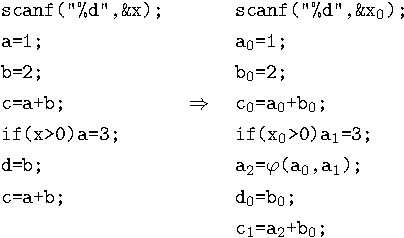
\includegraphics{figures/SSA-example1-crop.pdf}
    \end{center}
\end{figure}

この例では，変換前の変数に対して更新される毎に添字を更新して変数を新たに割り当てる．
更新を一回に限定することで，添字が同じ変数は，実行フローにおいて同じ値を持つことが保証される．
\verb|b|は，最初に2に更新された後，このプログラムの中では更新されることがないので，
\verb|b|$_0$が最後まで用いられるので，この値が伝播していることがわかる．\verb|a|$_0$
は，最初に1に更新され，再度更新されると\verb|a|$_1$に変数名を変えて，3に更新する．
ここでは，\verb|x|に入力される値は，ユーザーからの入力なのでプログラムを走らせないと
わからない．この入力に応じて，最終行の\verb|a|は，1または3の値となり，プログラムだけで
どちらの値になるか不明であるが，どちらかの値になることは解析できる．SSAでは，このような
静的に解析できないフローに対して$\varphi$という特別な関数の形で表す．
このために\verb|a|$_2$という新たな変数を割り当て，$\varphi$\verb|(a|$_0$\verb|,a|$_1$\verb|)|
によって値を更新する．$\varphi$関数は，評価する対象でなく，いずれかの選択が実行時になされる
ことを表現している．

ループを持つ場合においても，データのフローを単一代入の形で表すことができる．

\begin{figure}[H]
    \begin{center}
        \begin{tabularx}{\textwidth}{m{.6\textwidth}m{.3\textwidth}}
            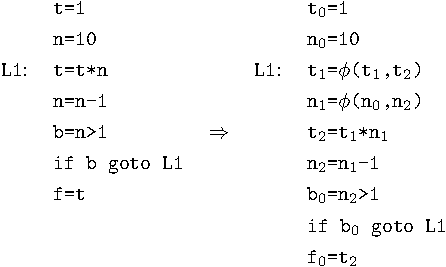
\includegraphics{figures/SSA-example2-crop.pdf}
             &
            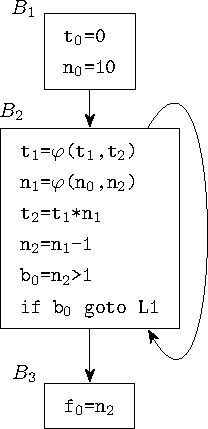
\includegraphics{figures/SSA-example2-CFG-crop.pdf}
        \end{tabularx}
    \end{center}
    \caption{ループを含むプログラムのSSAへの変換とフローグラフ}\label{fig:SSAwithLoop}
\end{figure}

ここでは，\verb|L1|の時点で，ループ内の変数は，ループに入る前のデータか，ループの繰り返しからくるデータなのかプログラムからはわからない．\verb|t=t*n|の右辺の\verb|t|は，\verb|t|$_0$か\verb|t|$_2$のどちらかである．

\subsection{$\varphi$関数}

SSA形式のプログラムに変換するためには，プログラムから解析可能な各変数の依存関係を計算し，
依存関係が実行によって決まるポイントに$\varphi$関数を挿入する．以下に，$\varphi$関数を挿入する
場所を決定する手法について示す．

ここで，コントロールグラフは，有向グラフ$(V,E,v_{init})$として与えられているとする．

\begin{Def}[定義合流条件]\label{def:definitionConfluence}
    変数$x$に対する$\varphi$関数が頂点$v$に挿入されるための必要十分条件は，以下に示す条件(1)$\sim$(4)を満たす
    コントロールグラフ上の路$p:v_0\rightarrow v_1\rightarrow\cdots\rightarrow v_k$,
    $q:u_0\rightarrow u_1\rightarrow\cdots\rightarrow u_\ell$が存在することである．
    \begin{list}{(\arabic{coffee})}{\usecounter{coffee}}
        \item 路の長さが1以上である．($k>0$,$\ell>0$);
        \item $v_1$と$u_1$の両方に$x$の定義が存在する．;
        \item 路の終点$v$が一致している．($v_k=v_\ell=v$);
        \item 路の途中で交わることがない．($\{v_1,\cdots,v_{k-1}\}\cap\{u_1,\cdots,v_{\ell-1}\}=\varnothing$)
    \end{list}
\end{Def}

頂点に$\varphi$関数が挿入されて，$x=\varphi(x,\cdots,x)$が頂点$v$に挿入されると，新たなコントロールフローグラフが得られるため，
この更新されたグラフに対して繰り返して上記の条件をチェックする必要がある．図\ref{flg:flowgraph}の変数\verb|t|に関して，
$v_0=B_1$, $u_0=B_2$, $v=B_2$とすると$B_1\rightarrow B_2$と$B_2\rightarrow B_2$であるため，
定義合流条件を満たす．$B_2$に$\varphi$関数\verb|t=|$\varphi$\verb|(t,t)|
が挿入される．\verb|n|についても同様である．これらの挿入によって，新たなフローは生じないのでこれ以上$\varphi$関数を挿入する必要はない．
定義\ref{def:definitionConfluence}に沿って$\varphi$関数を挿入するためには
コントロールフローグラフの路を網羅的に検査すればよい．

\begin{tcolorbox}[title={$\varphi$関数の挿入}]
    変数\verb|x|に対して定義\ref{def:definitionConfluence}の条件を満たす$v_0$, $u_0$, $v$がフローグラフに存在し，頂点$v$の基本ブロックに
    $\varphi$関数が含まれていないならば，$v$に\verb|x=|$\varphi$\verb|(x,...,x)|を挿入する．\\
    定義合流条件を満たす$v_0$, $u_0$, $v$ がなくなるまで，上記を繰り返す．
\end{tcolorbox}

\begin{figure}
    \centering
    \begin{tabularx}{\linewidth}{m{.25\linewidth}cm{.25\linewidth}cm{.25\linewidth}}
        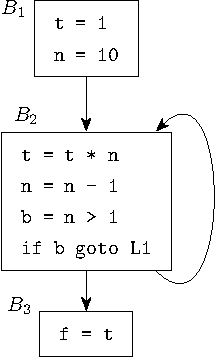
\includegraphics[width=\linewidth]{figures/phi-insertion-example-crop.pdf}
                                      & $\Rightarrow$ &
        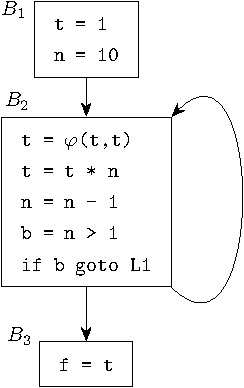
\includegraphics[width=\linewidth]{figures/phi-insertion-example-1-crop.pdf}
                                      & $\Rightarrow$ &
        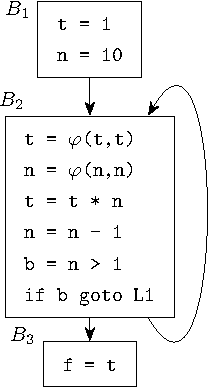
\includegraphics[width=\linewidth]{figures/phi-insersion-example-2-crop.pdf}                     \\[3.5cm]
        {\bf 合流定義条件:}                 &               & {\bf 合流定義条件:}                 &  & {\bf 合流定義条件:} \\
        \verb|t|:$v_0=B_1$,$u_0=v=B2$ &               & \verb|u|:$v_0=B_1$,$u_0=v=B2$ &  &               \\
        \verb|u|:$v_0=B_1$,$u_0=v=B2$ &               &                               &  &
    \end{tabularx}
    \caption{$\varphi$関数の挿入}\label{fig:phiFuncInsert}
\end{figure}

フローグラフにおいて，条件の適用をチェックして$\varphi$関数を挿入する方法をそのまま実装しようとすると，グラフの頂点の組み合わせ$(v_0,u_0,v)$を尽くして，頂点間の到達可能性と合流可能性を毎回チェックする必要があり，効率的とは言えない．コンパイラへの実装においては，有向グラフの支配関係を用いたより効率のよい挿入アルゴリズムが用いられる．

\begin{Def}
    フローグラフを$(V,E,v_{init})$とする．
    頂点$v,u$に対して，$v_{init}$から$u$へのすべての路に
    おいて$v$が出現するとき，$v$は$u$の{\bf 支配頂点(dominator)}であると呼び，$u\domll v$と書く．
    $u\not= v$かつ$u\domll v$であるとき，$u\ll v$と書く．
    $u$の支配頂点の集合$\domv{u}=\{v\;|\;u\domll v\}$で定義する．
\end{Def}

どの頂点$v$についても$v_{init}\in\domv{v}$かつ$v\in\domv{v}$である．$\domll$は半順序である．
\begin{itemize}
    \item (反射律) $v\domll v$
    \item (反対称律) $v\domll u$かつ$u\domll v$ならば$u=v$
    \item (推移律) $v\domll u$かつ$u\domll w$ならば$v\domll w$
\end{itemize}

$u\not= v_{init}$のとき，$\domv{u}\backslash\{u\}$には$\domll$の意味で最小の頂点が一つ存在する．
もし複数の頂点$v_1,v_2\in\domv{u}\backslash\{u\}$が存在したとすると，$v_1$, $v_2$はともに$v_{init}$から$u$の
すべての路に出現することになるため，$v_1\domll v_2$, $v_2\domll v_1$となるので，
反対称律から$v_1=v_2$でなければならない．$v_{init}$から$v_{init}$に長さ0の路があるので，
$\domv{v_{init}}=\{v_{init}\}$であり，$\domv{v_{init}}\backslash\{v_{init}\}=\varnothing$なので
以上のような最小頂点は存在しない．$u\not=v_{init}$のとき，$\domv{u}\backslash\{u\}$の中の最小頂点を
$\idomv{u}$と書くことにする．このとき，$\idomv{v}\rightarrow\cdots\rightarrow v$である．

フローグラフ$G=(V,E,v_{init})$に対して，$u$に対する親ノードを$\idomv{u}$とする辺$D=\{(\idomv{v},v)\}$
から構成される有向グラフ$T=(V,D)$は，$v_{init}$から$V$の各頂点
への路が存在することから，$v_{init}$を根とする木構造が構成される\footnote{$v_{init}$は$\mathsf{idom}$をもたないことから，親となる頂点がない}．
この木構造$T$を$G$に対する{\bf 支配木(dominator tree)}という．

\begin{Exmp}
    図\ref{fig:DTexample}に支配木の構成例を示す．$v_{init}=v_1$とすると$v_7$については，
    $v_1\rightarrow v_2\rightarrow v_3\rightarrow v_5\rightarrow v_7$,
    $v_1\rightarrow v_2\rightarrow v_3\rightarrow v_6\rightarrow v_6$ の２つの路があるので，
    $\idomv{v_7}=v_3$となる．
    \begin{figure}[t]
        \begin{center}
            \begin{tabularx}{.85\linewidth}{m{.2\linewidth}m{.45\linewidth}m{.2\linewidth}}
                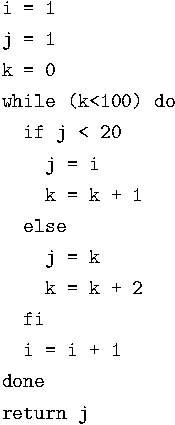
\includegraphics{figures/SSA-example3-prog-crop.pdf}
                                               &
                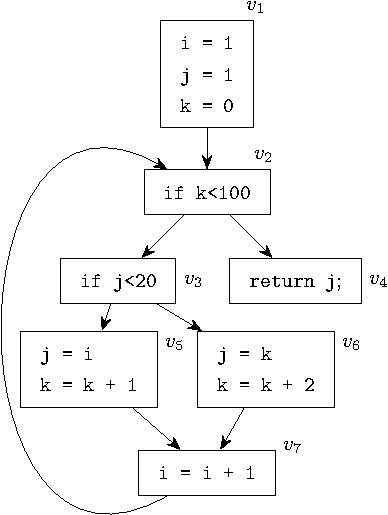
\includegraphics{figures/SSA-example3-CFG-crop.pdf}
                                               &
                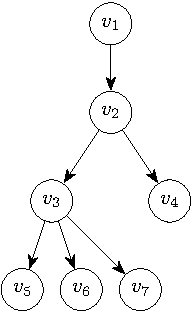
\includegraphics{figures/SSA-example3-DTree-crop.pdf} \\
                \multicolumn{1}{c}{(a) プログラム}  &
                \multicolumn{1}{c}{(b) フローグラフ} &
                \multicolumn{1}{c}{(c) 支配木}
            \end{tabularx}
        \end{center}
        \caption{支配木の例}\label{fig:DTexample}
    \end{figure}
\end{Exmp}

% SSA形式においては以下の性質が成り立っている．

% \begin{enumerate}
% \item\label{SSAPropOne} \verb|x|が$\varphi$関数の$i$番目の引数であるとき，その\verb|x|を定義している頂点は
% $\varphi$関数を含む頂点の$i$番目の先行頂点である．
% \item \verb|x|が$\varphi$関数以外で頂点$v$で参照される場合，その定義をしている頂点が$v$を支配する．
% \end{enumerate}

頂点$v,u$に対して，$u\not=v$かつ$u\domll v$であるとき，$v$は$u$を{\bf 真に支配する}といい，$u\ll v$と書くことにする．
\begin{Def}\label{def:DominanceFrontier}
    フローグラフ$(V,E,v_{init})$が与えられたとき，$v\in V$の{\bf 支配辺境(dominance frontier)}$DF(v)$を
    以下のように定義する．
    \[DF(v)=\{u\in V\;|\;\mbox{適当な$w$が存在して} w\domll v\mbox{ かつ }u\not\ll v\mbox{ かつ }w\rightarrow u\}\]
\end{Def}

支配辺境$DF(v)$は，直前の頂点までは$v$に支配されているが，$v$の支配が及ばない頂点の集合である．$v$において変数\verb|x|の
定義があれば，$DF(v)$の頂点において\verb|x|の$\varphi$関数を挿入する必要がある．
$\varphi$関数は新たな定義を生むため，新たな$\varphi$関数の挿入が生じないようになるまで，各$DF(v)$に$\varphi$関数を挿入する必要が生じる．ここで，支配木構造に着目すれば，各頂点に
対して１回だけ$\varphi$関数の挿入をチェックすればよいことが示される．

\begin{Lem}\label{lem:DFcomp}
    \begin{itemize}
        \item $DF_{local}(v)=\{u\;|\;v\rightarrow u,\idomv{u}\not= v\}$
        \item $DF_{up}(v)=\{u\in DF(v)\;|\;u\not\ll\idomv{v}\}$
    \end{itemize}
    とするとき，
    \[ DF(v)=DF_{local}(v)\cup\bigcup_{w\in\mathsf{Child}(v)}DF_{up}(w) \]
    ここで，$\mathsf{Child}(v)=\{w\;|\;\idomv{w}=v\}$
\end{Lem}

この補題の証明は本章の最後に付録として示す．補題\ref{lem:DFcomp}に沿って
$DF_{up}(v)$を計算しようとすると，
$\idomv{w}=v$であるような$w$の$DF(w)$を計算しておく必要がある．
$\mathsf{idom}$が支配木を構成することに注目すれば，
支配木を深さ優先で探索して，各頂点$v$に対する$DF(v)$を
計算できることがわかる．(アルゴリズム\ref{alg:dominanceFrontier})



\begin{algorithm}[t]
    \centering
    \begin{minipage}{.7\textwidth}
        \begin{algorithmic}
            \caption{支配辺境の計算}\label{alg:dominanceFrontier}
            \Procedure{computeDF}{$n$}
            \State $S \gets \{\}$
            \ForAll{$y \in \mathsf{succ}[n]$}   \Comment $DF_{local}$の計算
            \If{$\idomv{y}\not=n$}
            \State $S \gets S\cup\{y\}$
            \EndIf
            \EndFor
            \ForAll{$c \in \mathsf{Child}(n)$}  \Comment $DF_{up}$の計算
            \State computeDF(c) \Comment 支配木の子頂点から計算する
            \ForAll{$w \in DF[c]$}
            \If{$w\notin\domv{n}$ or $n=w$}
            \State $S\gets S\cup\{w\}$
            \EndIf
            \EndFor
            \EndFor
            \State $DF[n]\gets S$
            \EndProcedure
        \end{algorithmic}
    \end{minipage}
\end{algorithm}

ここで，$\mathsf{succ}[n]=\{v\;|\;n\rightarrow v\}$である．

\begin{Exmp}
    図\ref{fig:DTexample}のフローグラフに対して，各頂点の支配辺境を次のように求められる．
    まず支配木の葉頂点として$\{v_5,v_6,v_7\}$の$DF_{local}$を計算する．
    支配木の葉頂点においては，$\mathsf{Child}(v)=\varnothing$であり，
    $DF_{local}(v_4)=DF(v_4)=\varnothing$,$DF_{local}(v_5)=DF(v_5)=\{v_7\}$,
    $DF_{local}(v_6)=DF(v_7)=\{v_7\}$, $DF_{local}(v_7)=DF(v_2)=\{v_2\}$.

    $DF(v_3)=DF_{local}(v_3)\cup DF_{up}(v_5)\cup DF_{up}(v_6)\cup DF_{up}(v_7)$.

    $DF_{up}(v_5)=DF_{up}(v_6)=\{u\in DF(v_5)|u\not\ll v_3)\}=\varnothing$,
    $DF_{up}(v_7)=\{u\in DF(v_7)|u\not\ll v_3\}=\{v_2\}$
    $DF_{local}(v_3)=\varnothing$ であり，$DF(v_3)=DF_{up}(v_5)\cup DF_{up}(v_6)\cup DF_{up}(v_7)=\{v_2\}$.

    $DF_{local}(v_2)=\varnothing$, $DF(v_2)=DF_{up}(v3)\cup DF_{up}(v4)=\{v_2\}$
    $DF_{up}(v_2)=\{u\in DF(V_2)|u\not\ll v_1\}=\varnothing$

    $DF_{local}(v_1)=\varnothing$より$DF(v_1)=DF_{up}(v_2)=\varnothing$となる．
    \begin{center}
        \begin{tabular}{|c|c|c|c|}\hline
            $v$   & $DF_{local}$  & $DF_{up}$     & $DF$          \\\hline
            $v_1$ & $\varnothing$ & $\varnothing$ & $\varnothing$ \\\hline
            $v_2$ & $\varnothing$ & $\varnothing$ & $\{v_2\}$     \\\hline
            $v_3$ & $\varnothing$ & $\varnothing$ & $\{v_2\}$     \\\hline
            $v_4$ & $\varnothing$ & $\varnothing$ & $\varnothing$ \\\hline
            $v_5$ & $\{v_7\}$     & $\varnothing$ & $\{v_7\}$     \\\hline
            $v_6$ & $\{v_7\}$     & $\varnothing$ & $\{v_7\}$     \\\hline
            $v_7$ & $\{v_2\}$     & $\{v_2\}$     & $\{v_2\}$     \\\hline
        \end{tabular}
    \end{center}
\end{Exmp}

変数\verb|x|の$\varphi$関数は頂点$v$に挿入される条件は定義合流条件による．
変数の定義を含む頂点の集合を$S$とすると，定義\ref{def:definitionConfluence}は
次のようになる．

\begin{tcolorbox}[title={定義合流条件(S)}]
    $u_0,w_0\in S$に対して，長さ１以上で途中で交わらずに$v$で合流する路$p$:$u_0\rightarrow\cdots\rightarrow u_k=v$,
    および$q$:$w_0\rightarrow\cdots\rightarrow w_\ell=v$が存在する．($\{u_0,\cdots,u_k\}\cap\{w_0,\cdots,w_\ell\}=\varnothing$)
\end{tcolorbox}

$S$に対してこの条件を満たす合流頂点$v$の集合を$J(S)$とする．

変数\verb|x|の定義をもつ頂点集合を$S^{\texttt{x}}_0$とする．$J(S^{\texttt{x}}_0)$は，$\texttt{x}$に対する$\varphi$関数を
最初に挿入する頂点である．$J(S^{\texttt{x}}_0)=S^{\texttt{x}}_1$では$\varphi$関数の挿入は$\texttt{x}$の定義を生むので，
$J(S^{\texttt{x}}_0\cup S^{\texttt{x}}_1)$が\verb|x|の定義を含む頂点の集合となる．

$S^x_{i+1}=J(S^x_0\cup S^x_i)$とすると$S^x_0,S^x_1,S^x_2,\cdots $により変数$x$の$\varphi$関数を挿入する頂点を数え上げることができる．
$S^x_{i}\subseteq S^x_{i+1}$であり，フローグラフの頂点は有限個であることから，$i$の増加によって変化しなくなるときの集合を$J^+(S^x_0)$とする．
$J^+(S^x_0)$は$DF$によって求めることができる．

\begin{Thm}\label{thm:DFlimit}
    頂点の集合$S_0$に対して
    $DF(S_0)=\bigcup_{v\in S_0}DF(v)$とする．$F_i$の系列を以下のように定義する．
    \begin{eqnarray*}
        F_0 & = & \varnothing\\
        F_{i+1} & = & DF(S_0\cup F_i)
    \end{eqnarray*}
    $DF(S_0\cup F_i)=DF(S_0)\cup DF(F_i)$であることから$F_i$の系列は単調に増加する．この系列が変化しなくなるまで
    $i$を増加させて得られる頂点集合を$DF^+(S_0)$とする．

    このとき$DF^+(S_0)=J^+(S_0)$である．
\end{Thm}

この定理の証明については，文献\cite{DBLP:journals/toplas/CytronFRWZ91}を参照．

\begin{Exmp}\label{example:phiFunc}
    以下に$\varphi$関数の挿入の例を示す．

    \vspace*{10pt}

    \begin{tabularx}{\linewidth}{m{.2\linewidth}m{.5\linewidth}m{.2\linewidth}}
        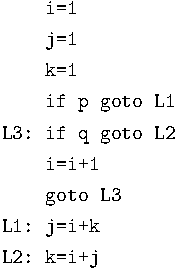
\includegraphics{figures/SSA-example4-prog-crop.pdf}
                  &
        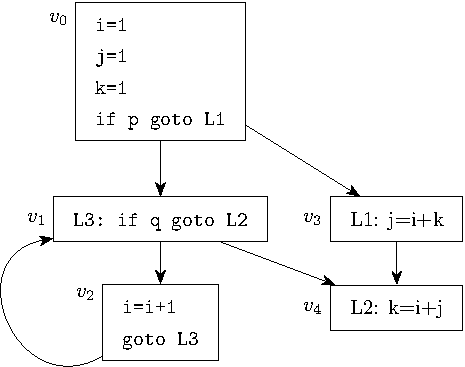
\includegraphics[width=\linewidth]{figures/SSA-example4-CFG-crop.pdf}
                  &
        \begin{center}
            \begin{tabular}{|l|l|}\hline
                $v$   & $DF(v)$       \\\hline\hline
                $v_0$ & $\varnothing$ \\\hline
                $v_1$ & $\{v_1,v_4\}$ \\\hline
                $v_2$ & $\{v_1\}$     \\\hline
                $v_3$ & $\{v_4\}$     \\\hline
                $v_4$ & $\varnothing$ \\\hline
            \end{tabular}\end{center} \\
        (a) プログラム & (b) フローグラフ & (c) 支配辺境
    \end{tabularx}

    \vspace*{10pt}

    各変数の合流条件は以下のように計算される．

    \[
        \begin{array}{|l||l|l|l|}\hline
            S_0 & S^{\texttt{i}}_0=\{v_0,v_2\}              & S^{\texttt{j}}_0=\{v_0,v_3\}         & S^{\texttt{k}}_0=\{v_0,v_4\}     \\
                & DF(S^\texttt{i}_0)=\{v_1\}                & DF(S^\texttt{j}_0)=\{v4\}            & DF(S^\texttt{k}_0)=\varnothing   \\\hline
            S_1 & DF(S^\texttt{i}_0\cup\{v_1\})=\{v_1,v_4\} & DF(S^\texttt{j}_0\cup\{v_4\})=\{v4\} & DF(S^\texttt{k}_0)=\varnothing   \\
                & DF(S_0\cup\{v_1,v_4\})=\{v_1,v_4\}        &                                      &                                  \\\hline
                & DF^+(S^\texttt{i}_0)=\{v_1,v_4\}          & DF^+(S^\texttt{j}_0)=\{v_4\}         & DF^+(S^\texttt{k}_0)=\varnothing \\\hline
        \end{array}
    \]

    したがって，$v_1,v_4$の先頭に$\texttt{i}$の$\varphi$関数，$v_4$の先頭に$\texttt{j}$の$\varphi$関数を挿入する．

    \begin{center}
        \begin{tabular}{cc}
            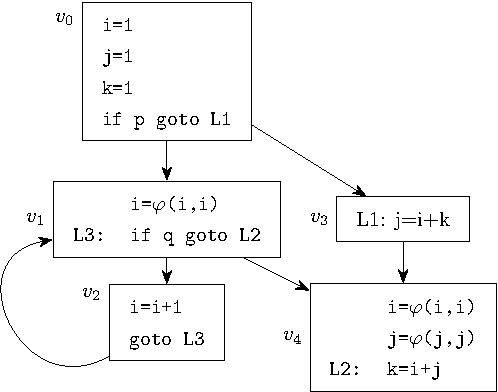
\includegraphics{figures/SSA-example4-phi-crop.pdf}
                           &
            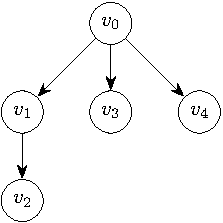
\includegraphics{figures/SSA-example4-DTree-crop.pdf} \\
            $\varphi$関数の挿入 & 支配木
        \end{tabular}
    \end{center}

\end{Exmp}

\subsection{SSA形式への変換}

$\varphi$関数を挿入した後，各変数に添字を付加して各３番地命令をSSA形式に変換する．フローグラフを支配木によってトラバースすることによってフローに従って字を付加する．

各変数$x$について，まず左辺で定義する変数に添字をつけ，新たに定義される
まで右辺で参照する変数にその添字をつける．アルゴリズムをアルゴリズム\ref{alg:RenameForSSA}に示す．

例\ref{example:phiFunc}に対してアルゴリズムを適用する．
\begin{trivlist}
    \item[{\bf 初期化:}] 各変数$\tti$, $\ttj$, $\ttk$に対して，カウンタを$0$にセットして，スタック$\mathsf{Stack}[x]$に$0$をプッシュする．
    \item[{\bf Step1:}] $\mathsf{Count}[\tti]=\mathsf{Count}[\ttj]=\mathsf{Count}[\ttk]=1$とし，$\textsc{Rename}(v_0)$において，9行目から13行目で，$\tti$, $\ttj$, $\ttk$の左辺に添字$1$をつける．\\
    $v_0$の後続頂点のうち，$v_1$に対して，16行目から20行目を適用する．$v_0$を$v_1$の１番目の先行頂点とする．$(j=1)$ \\
    $\tti=1$であるので，
    $v_1$の$\tti\tteq\varphi(\tti,\tti)$を$\tti\tteq\varphi(\tti_1,\tti)$におきかえる．
    $v_3$には$\varphi$関数が含まれない．\\
    $v_0$の支配木の子頂点$v_1$を選んで$\textsc{Rename}(v_1)$を呼び出す．
    \item[{\bf Step2:}]
    $v_1$において，$\varphi$関数以外で参照される変数はなく，$\tti$が定義されるので，10行目から13行目のブロックにおいて，$\mathsf{Count}[\tti]$をインクリメントして，
    $\tti_2\tteq\varphi(\tti_1,\tti)$とする．\\
    15行目から22行目までの実行で，$v_4$において，
    $\varphi$関数内の$\tti$と$\ttj$の参照を置換して，
    $\tti\tteq\varphi(\tti,\tti_1)$,
    $\ttj\tteq\varphi(\ttj_1,\ttj)$とする．
    (フローグラフでは$v_4$は$v_1$の1番目の後続頂点である．)\\
    24行目で，$v_1$の支配木における子頂点は$v_2$なので，$\textsc{Rename}(v_2)$を呼び出す．
    \item[{\bf Step3:}] $v_3$において，4行目から7行目の適用によって，
    $\tti\tteq\tti_2\ttpl 1$となる．つぎに，$v_3$では，$\tti$が定義されているので，$\mathsf{Count}[\tti]$を増やして，
    $\tti_3\tteq\tti_2\ttpl 1$とする．
    この時点で，$\mathsf{Count}[\tti]=3$,$\mathsf{Stack}[\tti]=[3,2,1,0]$\\
    $v_2$は支配木の子頂点を持たないので，26行目から30行目のループが実行される．$v_2$で定義された変数は$\tti$なので，ポップし，
    $\mathsf{Stack}[\tti]=[2,1,0]$とする．
    \item[{\bf Step2':}] Step2の$\textsc{Rename}(v_2)$が終了したので，
    その後の26行目から30行目を実行する．
    $v_2$で$\tti$が$\varphi$関数で定義されたので$\mathsf{Stack}[\tti]$をポップして，$\mathsf{Stack}[\tti]=[1,0]$とする．
    \item[{\bf }] Step1の23行目で，支配木の次の子頂点$v_3$を選んで$\textsc{Rename}(v_3)$を呼び出す．
    \item[{\bf Step4:}] 4行目から7行目のループで$\mathsf{Stack}[\tti]=\mathsf{Stack}[\ttj]=[1,0]$であることから，$\ttj\tteq\tti_1\ttpl\ttj_1$に置換する．
    9行目から14行目のループで，$\ttj$が左辺で定義されているので，
    $\mathsf{Count}[\ttj]$をインクリメントし，$\mathsf{Stack}[\ttj]=[2,1,0]$としたあと，$\ttj_2\tteq\tti_1\ttpl\ttk_1$とする．
    15行目から22行目のループにおいて，$v_4$は$v_3$の後続頂点であり，$v_3$は$v_4$にとって2番目の先行頂点であるので，$v_4$の$\varphi$関数の２番目の引数を置き換えて，$\tti\tteq\varphi(\tti_2,\tti_1)$,
    $\ttj\tteq\varphi(\ttj_1,\ttj_2)$とする．\\
    $v_3$には支配木の子頂点はなく，$\ttj$を定義したので，$\mathsf{Stack}[\ttj]$をポップして，$[1,0]$とする．
    この時点で，$\mathsf{Count}[\tti]=3$, $\mathsf{Count}[\ttj]=2$である．
    \item[{\bf Step1'':}] 23行目で３番めの子頂点として$v_4$を選択して，$\textsc{Rename}(v_4)$を呼び出す．
    \item[{\bf Step5:}] 2行目から15行目までのループで順に置換する．\\
    $\tti_4\tteq\varphi(\tti_2,\tti_1)$
    ここで，$\mathsf{Stack}[\tti]=[4,1,0]$, $\mathsf{Count}[\tti]=4$\\
    $\ttj_3\tteq\varphi(\ttj_1,\ttj_2)$
    ここで，$\mathsf{Stack}[\ttj]=[3,1,0]$, $\mathsf{Count}[\ttj]=3$\\
    最後に$\ttk$が新たに定義されるので，$\ttk_2\tteq\tti_4\ttpl\ttj_3$と置換される．
\end{trivlist}

図\ref{fig:SSAexample}に適用結果を示す．
\begin{figure}
    \centering
    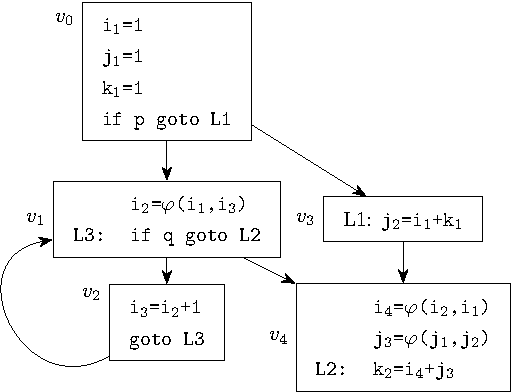
\includegraphics{figures/SSA-example4-SSA-crop.pdf}
    \caption{例\ref{example:phiFunc}に対するアルゴリズム2の適用結果}\label{fig:SSAexample}
\end{figure}

\begin{algorithm}[t]
    \caption{SSAへの変換}\label{alg:RenameForSSA}
    \begin{tabularx}{\textwidth}{m{.3\textwidth}m{.5\textwidth}}
        \begin{minipage}{.4\textwidth}
            /* 初期化 */
            \begin{algorithmic}
                \ForAll{$a\ \in Var$}
                \State $\mathsf{Count}[a]\leftarrow 0$
                \State $\mathsf{Stack}[a]\leftarrow \varnothing$
                \State $\mathsf{Stack}[a]$に$0$をプッシュ
                \EndFor
            \end{algorithmic}
        \end{minipage}
         &
        \begin{minipage}{.6\textwidth}
            \begin{algorithmic}[1]
                \Procedure{Rename}{$n$}
                \ForAll{$S$\ in ブロック$n$}
                \If{$S$が$\varphi$関数でないとき}
                \ForAll{$x$ in $S$で参照される変数}
                \State $i\leftarrow top(\mathsf{Stack}[x])$
                \State $S$の$x$の参照を$x_i$で置き換える
                \EndFor
                \EndIf
                \ForAll{$S$の左辺で定義される変数$a$}
                \State $\mathsf{Count}[a]\leftarrow\mathsf{Count}[a]+1$
                \State $i\leftarrow\mathsf{Count}[a]$
                \State $\mathsf{Stack}[a]$に$i$をpush
                \State $S$の左辺の$a$を$a_i$で置き換える
                \EndFor
                \EndFor
                \ForAll{$Y$ in ブロック$n$の後続頂点}
                \State $n$は$Y$の$j$番目の先行頂点
                \ForAll $Y$に含まれる$\varphi$関数
                \State $\varphi$関数の$j$番目の引数が$a$のとき\\
                \hspace*{7em}$i\leftarrow top(\mathsf{Stack}[a])$
                \State $\varphi$関数の$j$番目の引数の$a$を$a_i$に置換
                \EndFor
                \EndFor
                \ForAll{$X$ in 支配木における$n$の子頂点}
                \State call \textsc{Rename}($X$)
                \EndFor
                \ForAll{ブロック$n$の$S$}
                \ForAll $a$ in $S$における定義
                \State $\mathsf{Stack}[a]$をポップ
                \EndFor
                \EndFor
                \EndProcedure
            \end{algorithmic}
        \end{minipage}
    \end{tabularx}
\end{algorithm}

\subsection{SSA上での最適化}

SSA形式に変換することによって，手続き内において基本ブロックにとらわれない最適化が可能になる．

\paragraph{不要コード除去}

SSA形式における不要コード除去は，変数名によってどの定義によって変数が三sh要されているかがわかる．左辺で定義されている変数が右辺で参照されていない（あるいは何等かの副作用を及ぼさない）場合は，その定義を除去しても意味は変わらない．

\paragraph{定数伝播}

SSA形式であれば，同じ変数名であるとき同じ値を持つ．$x_i\leftarrow c$という定数$c$の代入があれば，$x_i$は$c$に置き換えることができる．もし，
$x_k=\varphi(x_1,\cdots,x_n)$において，$x_1,\cdots,x_n$がすべて
同じ定数に置き換えられた場合は，$x_k$もその定数に置き換えて伝播させることができる．

同じ手続きの中(intra-procedure)であれば，コピー伝播，ループ変数の畳み込み，共通部分式除去などの方法を基本ブロックを意識せずに適用することができる．手続きにまたがる(inter-procedure)最適化はさらに解析が必要となる．

\paragraph{支配関係の保存}

SSAによる最適化においては，変換前と変換後がそれぞれ支配関係を保存することを要求する\footnote{前後で同じ支配関係である必要はない．}\cite{TigerBook}．図\ref{fig:DominacePreservation}のようなフロー
グラフを(a)から(b)に変換することを考える．$v_1$と$v_3$,$v_3$と$v_4$の間に$\ttz$が更新されることがないとすると，$v_1$と$v_4$の分岐条件は変わらないので，(b)のようにしても意味は変わらない．$v_5$の$\ttx$は(a)では，$v_3$で定義された値，(b)では，$v_1$で定義された値である．(b)では，$v_1$は$v_5$を支配しない．

このような最適化は$v_1$と$v_4$における$\ttz<0$の評価が変わらないことが保証されれば正しい．これを保証するためには，実行フローが同じであることを証明しなければならず，このような解析は一般には決定可能でない．

SSA形式では，変数の代入による定義が唯一であるという条件の他に，「変数定義が変数使用を支配する」という条件も成り立っている必要がある．SSA形式による最適化手法では，この条件によってフローグラフの構造から可能な最適化を行い，すべての最適化を可能とするものではない．

\begin{figure}[t]
    \begin{center}
        \begin{tabular}{ccc}
            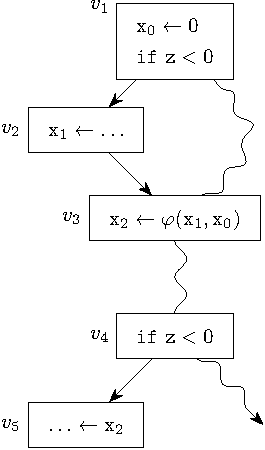
\includegraphics[scale=0.75]{figures/SSA-dominance-break-crop.pdf}
                    &  &
            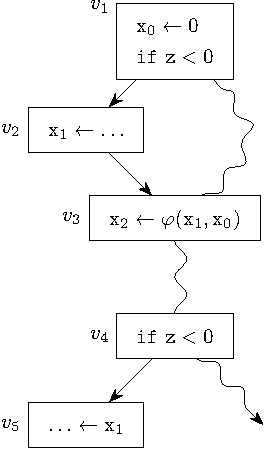
\includegraphics[scale=0.75]{figures/SSA-dominance-break-after-crop.pdf} \\
            (a)最適化前 &  & (b)最適化後
        \end{tabular}
    \end{center}
    \caption{支配関係を壊す変換}\label{fig:DominancePreservation}
\end{figure}

\subsection{$\varphi$関数を持たないSSA形式への変換}

$\varphi$関数は実行可能な関数ではないので，コンパイルをすすめるためには，$\varphi$関数を消去した等価なプログラムに変換する必要がある．
$\varphi$関数は頂点$v$の基本ブロックの先頭に挿入される．$x_3=\varphi(x_1,x_2)$が先頭に挿入されている場合，$x_1$，$x_2$に対応するフローグラフ上の路において$v$の直前の頂点に$x_3=x_1$, $x_3=x_2$を
挿入すれば，$\varphi$関数を消去しても意味は変わらない．(図\ref{fig:phiElimination}) 各路の$v$への先行頂点$u$が$v$を唯一の
後続頂点として持つときは，新たに頂点は挿入せず，$u$の最後に
$x_3=x_1$ないしは$x_3=x_2$を追加する(図\ref{fig:phiElimination})．$u$の最後がgotoである
場合は，goto文の前に挿入する．唯一の先行頂点を持つ場合には，
さらにその前に挿入する\footnote{$\varphi$関数の挿入時には唯一の
    先行頂点を持つようなブロックは存在しない．最適化後には現れる可能性がある．}．

以上の方法で$\varphi$関数を消去するには，$\varphi$関数を含む頂点$v$の先行頂点が$v$を唯一の後続頂点として持つか，$v$が唯一の先行頂点を持つ必要がある．

$\varphi$関数を含むブロックの頂点がこの条件を満たさない場合は，$v$を唯一の後続頂点とする空の頂点を挿入することで，この条件を満たすフローグラフを構成できる．このフローグラフに上記の方法を適用して$\varphi$関数を消去可能である．

\begin{figure}
    \centering
    \begin{tabular}{cc}
        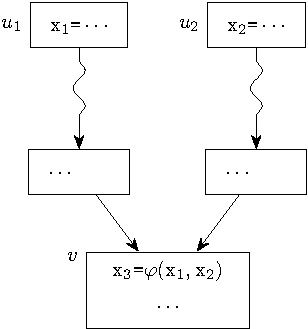
\includegraphics[width=.3\linewidth]{figures/SSA-phiElimination-a-crop.pdf}
         &
        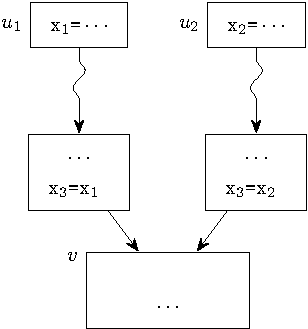
\includegraphics[width=.3\linewidth]{figures/SSA-phiElimination-b-crop.pdf}
    \end{tabular}
    \caption{SSA形式からの$\varphi$関数の消去}
\end{figure}

例えば図\ref{fig:SSAexample}のフローグラフでは，$v_1$は$\varphi$関数を含み，$v_1$の先行頂点のうち$v_0$は複数の後続頂点$v_1$, $v_3$を持ち，$v_1$の先行頂点も複数存在する．従って，$v_0$と$v_1$の間に新たな頂点$w_0$を挿入することで条件を満たす．$v_4$についても$v_2$が複数の後続頂点を
持つので，$v_1$から$v_4$の間に新たな頂点$w_1$を挿入することでこの条件を満たす．(図\ref{fig:nodeInsert})

\begin{figure}
    \centering
    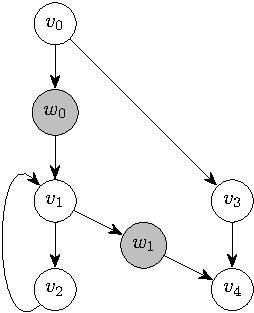
\includegraphics{figures/SSA-nodeInsert-crop.pdf}
    \caption{挿入条件を満たすために空頂点を追加}\label{fig:nodeInsert}
\end{figure}

\subsection*{[付録] 補題\ref{lem:DFcomp}およびアルゴリズム\ref{alg:dominanceFrontier}の証明}

\begin{repLem}{lem:DFcomp}
    \[
        DF(v)=DF_{local}(v)\cup\bigcup_{w\in\mathsf{Child}(v)}DF_{up}(w)
    \]
\end{repLem}
\begin{proof}
    \begin{trivlist}
        \item[($\supseteq$)] 定義\ref{def:DominanceFrontier}の定義式において，$w$として$v$をとると，$v\domll v$であるので，$DF_{local}(v)\subseteq DF(v)$である．$v$の子頂点$w$に対しては，$idom(w)=v$である．$v$の支配木の子頂点$w$に対して$DF_{up}(w)=\{u\;|\;\exists w':w'\domll u,u\not\ll w,w'\rightarrow u,u\not\ll\idomv{w}\}$.
        $DF(v)=\{u\;|\;\exists w':w'\domll v,u\not\ll v,w'\rightarrow u\}$. ここで，$w'\domll w$, $w\domll \idomv{w}$のとき，$w'\domll\idomv{w}$なので，$v=\idomv{w}$ならば$DF_{up}(w)\subseteq DF(v)$.
        よって右辺の要素はすべて$DF(v)$に含まれるから，$\supseteq$が示される．
        \item[($\subseteq$)]
        $x\in DF(v)$となる任意の頂点$x$に対して，$y\rightarrow x$であり$y\domll v$となる$y$が存在する．$y=v$ならば，
        $x\in DF_{local}(v)$である．$y\not=v$のときは，
        $y\ll v$であるので，$v$の支配木における子頂点$v'$が
        存在して，$y\domll v'$かつ$x\not\ll v'$. 定義から$x\in DF_{up}(v')$である．
    \end{trivlist}
\end{proof}

\begin{Lem}
    \[DF_{local}(v)=\{u\;|\;v\rightarrow u,\idomv{u}\not=v\}\]
\end{Lem}

\begin{proof}
    (作成中)
\end{proof}

\begin{Lem}
    頂点$v$と支配木における$v$の子頂点$w$に対して
    \[
        DF_{up}(w)=\{u\in DF(w)\;|\;\idomv{u}\not= v\}
    \]
\end{Lem}

\begin{proof}
    (作成中)
\end{proof}

\begin{Thm}
    アルゴリズム\ref{alg:dominanceFrontier}は$DF(v)$を正しく計算する．
\end{Thm}
\begin{proof}
    (作成中)
\end{proof}

\subsection*{[付録] 定理\ref{thm:DFlimit}の証明}

\begin{Lem}
    フローグラフにおいて，長さ１以上の路$p$: $v\rightarrow\cdots\rightarrow u$に対して，
    $p$上に，頂点$w\in\{v\}\cup DF^+(v)$が存在する．
    $p$上に$v$の支配頂点でない頂点があれば，$DF^+(v)$
    に属する．
\end{Lem}
\begin{proof}
    (作成中)
\end{proof}

\begin{Lem}
    フローグラフにおいて異なる頂点$u_1$, $u_2$を始点として$v$で合流する路$p$:$u_1\rightarrow\cdots\rightarrow v$, $q$:$u_2\rightarrow\cdots\rightarrow v$が存在するとき，$v\in DF^+(u_1)\cup DF^+(u_2)$である．
\end{Lem}
\begin{proof}
    (作成中)
\end{proof}

\begin{Lem}
    フローグラフの頂点集合$S$に対して，$J(S)\subseteq\cup_{v\in S}DF^+(v)$
\end{Lem}
\begin{proof}
    (作成中)
\end{proof}

\begin{Lem}
    $S$をフローグラフの始点を含む頂点集合とすると，
    $DF(S)\subseteq J(S)$
\end{Lem}
\begin{proof}
    (作成中)
\end{proof}

\begin{repThm}{thm:DFlimit}
    変数$x$に対する代入を含む基本ブロックに対する頂点集合を$S$とする．このとき，$DF^+(S)$は変数$x$の$\varphi$関数を挿入する頂点集合$J^+(S)$である．
\end{repThm}

\begin{proof}
    (作成中)
\end{proof}

\end{document}
